\chapter{ML-Modelle}
In dieser Arbeit wird die Device-Based Indoor-Lokalisation auf basis von Sensorwerten untersucht.
Das ist inspiriert von dem Orientierungssinn von Mensch und Tier.
Dabei werden diskrete Standorte unterschieden, sowie ob eine Anomalie entdeckt wurde,
d. h. ob das Modell sich an einem unbekannten Standort oder auf einem unbekannten Pfad befindet.
\newline
\newline
Abbildung \ref{fig:model_idea} zeigt die Architektur des verfolgten Ansatzes.
Zunächst werden aus den Sensorwerten Features extrahiert.
Die resultierende Feature-Menge wird dann von dem ML-Modell genutzt, um den Standort zu klassifizieren.
Zuletzt wird auf basis historischer Daten und dem Klassifizierungsergebnis in einem Analyseschritt (TODO: ML Ansatz?) bestimmt, ob eine Anomalie vorliegt.
Im Vergleich zu der Architektur von Mian \cite{naveedThesis} können die Klassifizierungsergebnisse bei der Feature-Extrahierung weiter verarbeitet werden.
\begin{figure}[h!]
    \centering
    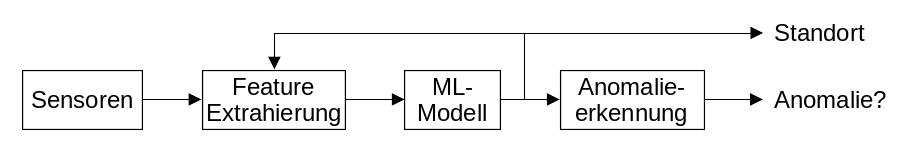
\includegraphics[width=\linewidth]{images/model_idea.png}
    \caption{Architektur des verfolgten Ansatzes.}
    \label{fig:model_idea}
\end{figure}
\newline
In dieser Arbeit Entscheidungsbaum basierte Klassifizierer mit KNN verglichen, insbesondere den von Mian verwendeten Ansatz mit FFNN.
Entscheidungsbäume sind deutlich effizienter als KNN, weswegen diese bei vergleichbarer Klassifizierungsgenauigkeit und Fehlertoleranz die preferierte Wahl sind.

\iffalse
Eigentlich eignen sich \textit{rekurrente neuronale Netze} (RNN) gut für diese Aufgabe, da serielle Daten verarbeitet werden
und zeitliche Abhängigkeiten für die Klassifizierung wichtig sind (TODO: Quelle).
Aber in dieser Arbeit wurde sich dagegen entschieden, da diese sehr rechenaufwändig sind und viel Speicher benötigen im Vergleich zu FFNN oder Entscheidungswälder,
weshalb diese suboptimal für kleine Mikrocontroller sind (TODO: Quelle).
\fi

\section{Standortenkodierung}
Als Standort wird ein einzigartiger diskreter Ort im Indoor-Szenario bezeichnet.
Bei der Klassifizierung können Standorte auf verschiedenen Arten im ML-Modell enkodiert werden.
Mian enkodierte die Pfade zwischen den Standorten, d. h. das Klassifizierungsergebnis ist der Pfad auf dem sich der Mikrocontroller befindet \cite{naveedThesis}.
\newline
\newline
Daneben wurden in dieser Arbeit noch zwei weitere Ansätze untersucht.
Im ersten Ansatz werden alle Punkte im Umkreis von bestimmten Punkten als Standorte definiert und alle restlichen als \textit{unbekannten Standort}.
Der zweite Ansatz kombiniert die beiden anderen Ansätze.
Zunächst werden, wie im ersten Ansatz, alle Punkte im Umkreis von bestimmten Punkten als Standorte definiert.
Dann werden die übrigen Punkte, also die Pfade zwischen zwei Standorten, als Standorte definiert.
\newline
\newline
Der Zusammenhang dieser Ansätze wird deutlich, wenn man eine Route als zyklischen Graphen betrachtet.
Einzigartige diskrete Punkte, die von interesse sind, bilden die Knoten und die Pfade zwischen diesen Punkten, die Kanten.
Mian's Ansatz nutzt nur die Kanten und folglich die anderen Ansätze jeweils die Knoten und die Knoten und Kanten.
\newline
\newline
Daraus wird die Komplexität und Genauigkeit dieser Ansätze deutlich.
Der Kantenansatz ist ein Kompromiss zwischen Genauigkeit und Komplexität.
Dabei bestimmt die Anzahl der zu klassifizierenden Standorte die Komplexität.
Zum einen ist gerade bei langen Pfaden eine geringe Auflösung im Vergleich zur Realposition zu erwarten,
d. h. es ist unklar, ob sich das Objekt am Anfang, Ende oder in dazwischen befindet.
Zum anderen werden in einem zyklischen Graphen mindestens so viele Standorte, wie beim Knotenansatz verwendet.
Der Knotenansatz benötigt am wenigsten Standorte zur Enkodierung ist aber außerhalb der Standorte sehr ungenau.
Aus einer Historie von vorherigen Standorten kann aber ein möglicher Pfad inferiert werden,
d. h. bei einer Gabelung können mehrere Pfade in Frage kommen.
Der kombinierte Ansatz bedarf enkodiert soviele Standorte wie beide Ansätze zusammen,
wodurch dieser Ansatz am komplexisten ist und am schlechtesten für große Routen skaliert.
Dafür ist die Auflösung des kombinierten Ansatzes so gut, wie eine diskrete Enkodierung es zulässt.
\newline
\newline
Ist in den aufgenommenen Trainingsdaten die Position des Objektes zum Zeitpunkt der Aufnahme der Sensorwerte bekannt,
so können die Standorte nach dem gewählten Enkodierungsansatz beliebig genau beschriftet werden.
Dies kann in einem Weiterverarbeitungsschritt nach der Aufnahme der Daten mit ein Karte von den Interessepunkten geschehen.
\newline
\newline
Bei der Evaluation in Kapitel \ref{sec:eval_anomalieerkennung} hat sich gezeigt, dass Anomalien besser erkannt werden können,
wenn die Auflösung des Enkodierungsansatzes hoch ist.
\section{Entscheidungswald}
\label{sec:model_dt}
Entscheidungsbaum basierte Klassifizierer sind sehr effizient und können trotzdem hohe Klassifizierungsgenauigkeiten bei hohen Fehlertoleranzen erreichen \cite{dymelThesis}.
Entscheidungswälder erhöhen die Klassifizierungsgenauigkeit während die Varianz reduziert wird, dafür wird aber der Speicherbedarf mit jedem Baum linear erhöht.
Der Klassifizierer soll zukünftig auf einem Mikrocontroller ausgeführt werden, d. h. die Größe des Entscheidungswaldes ist durch den Programmspeicher des Mikrocontrollers limitiert.
Zu dem Zeitpunkt, wo diese Arbeit verfasst wird, sind die Limitierungen des Mikrocontrollers noch nicht bekannt.
Für gewöhnlich ist der Programmspeicher aber auf wenige Kilo-Byte beschränkt \cite{dymelThesis}.
\newline
\newline
Als Ensemble-Methode wird \textit{RandomForest} benutzt, da dieser Entscheidungsbäume auf Basis von zufälligen Teilmengen der Feature-Menge konstruiert.
Dadurch ist eine erhöhte Toleranz gegenüber Fehlern, wie fehlerhafte Sensorwerte oder anderen Features zu erwarten.
\newpage
Um den Einfluss von verschiedenen Wald- und Baumgrößen auf die Fehlertoleranz und Klassifizierungsgenauigkeit hin zu untersuchen, werden verschiedene Größen
trainiert und auf den Testmengen evaluiert. Trotzdem wurden Dimensionen in einem Bereich gewählt, der für einen Mikrocontroller realistisch ist.
Es wurden jeweils Bäume und Wälder der Größe 8, 16, 32, und 64 untersucht.
\section{Feed Forward neuronales Netzwerk}
\label{sec:model_ffnn}
Für das KNN wird ein Feed Forward neuronales Netzwerk verwendet.
Das FFNN besteht aus drei bis sechs Schichten.
Alle Schichten, außer der letzten, verwenden ReLU als Aktivierungsfunktion.
Die letzte Schicht verwendet SoftMax.
\newline
\newline
Die Größe der Eingabeschicht ist abhängig von der Anzahl der verwendeten Features.
Die Features werden in einem Vorverarbeitungsschritt im Gegensatz zum Entscheidungswald normalisert.
Die Größe der Ausgabeschicht ist die Anzahl der verschieden diskreten Standorte, die unterschieden werden.
Je nach Konfiguration gibt es eins, zwei oder vier verdeckte Schichten, die jeweils 16, 32, 64 oder 128 Neuronen haben.
\newline
\newline
Die Standorte sind kategorische Daten, d. h. ihr Wert haben keine Aussage über die Beziehung der Standorte zueinander.
Aus diesem Grund werden sie kategorische Enkodiert, d. h. aus einem Wert $i$ aus $N$ möglichen Werten wird eine Liste der Größe $N$ generiert,
die überall 0 ist außer an der Stelle $i$, die 1 ist.
Folglich wird als Kostenfunktion \textit{kategorische Crossentropy} verwendet.
\newline
\newline
Als Lernalgorithmus wird Adam verwendet mit einer Batch-Größe von 50.
Trainiert wird über 75 Epochen.

\iffalse
\begin{itemize}
    \item Braucht man mehr Neuronen/Hidden Layer mit steigender Ort Anzahl?
\end{itemize}
\fi

\section{Feedback Kanten}
\begin{itemize}
    \item Was ist das?
    \item Wofür ist das Relevant?
    \item Wie funktioniert es?
    \item Wie wird das Problem umformuliert, für künstliche Rekurenz?
\end{itemize}

\section{Modell der Anomalieerkennung}
\begin{itemize}
    \item Wie funktioniert es?
    \item Welche Metriken werden verwendet?
\end{itemize}

\section{Training der Modelle}
\begin{itemize}
    \item Trainieren in Phasen => Erklären wie es genau funktioniert?
    \item Warum trainieren wir in Phasen? => Erkläre, dass wir Klassifizierungsfehler lernen wollen, damit wir wieder zurückfinden.
    \item Sag das wir die Zyklen der einzelnen Pfade nutzen
    \item Werden mehr Trainingsdaten benötigt mit steigender Ort Anzahl? Wenn ja wie viel?
    \item Doppeltes Trainieren nach Analyse der Feature Importance.
    \item Warum machen wir das so?
    \item Zufälliges Relabeling im Training? Warum und wie funktionierts?
    \item Anteil der Daten der gerelabelt wird steigt mit Anzahl der Zyklen
\end{itemize}
